\documentclass{article}
\usepackage[a4paper, margin=1in]{geometry}
\usepackage{amsmath, amssymb, amsthm}
\usepackage{graphicx}
\usepackage{titlesec}
\usepackage{hyperref}
\usepackage{physics}
\usepackage{tikz}
\usepackage{bbold}
\usepackage{caption}

\titleformat{\section}{\Large\bfseries}{\thesection}{1em}{}
\titleformat{\subsection}{\large\bfseries}{\thesubsection}{1em}{}

\title{\textbf{Cohomological Physics and Derived Hamiltonians:}\\
\large{A Logical Comparison to String Theory and M-Theory}}
\author{
  \textbf{Matthew Long}\\
  \textit{Magneton Labs}
}
\date{\today}

\begin{document}

\maketitle

\begin{abstract}
This paper explores the logical soundness of cohomological physics, derived Hamiltonians, and motivic cohomology as unifying frameworks for physics, biology, and computation. We analyze how these mathematical approaches compare to string theory and M-theory in terms of rigor, foundational assumptions, and physical implications. While string theory proposes physical entities like strings and branes, the cohomological approach models reality through algebraic and topological structures. Diagrams are provided to compare perturbative expansions in string theory with cohomological projections in derived Hamiltonian frameworks. We argue that cohomological physics offers a more mathematically complete foundation, although its physical interpretability and experimental predictions remain an open area of exploration. 
\end{abstract}

\section{Introduction}
The search for a unified theory that explains the fundamental forces of nature has led to the development of multiple theoretical frameworks. Among them, \textbf{string theory and M-theory} have dominated, offering a higher-dimensional description of particles and forces. However, these theories introduce conjectural elements such as extra dimensions and supersymmetry, which lack experimental verification.

An alternative approach lies in \textbf{cohomological physics}, where physical systems are modeled through algebraic structures such as derived categories, spectral sequences, and motivic cohomology. This paper explores whether cohomological physics, grounded in well-established mathematics, offers a more logically sound foundation compared to string theory and M-theory.

\section{Foundations of String Theory and Cohomological Physics}
\subsection{String Theory and Perturbative Expansions}
String theory postulates that elementary particles are one-dimensional strings vibrating in higher-dimensional space. M-theory generalizes this to include membranes (branes) and requires 11 dimensions to unify gravity with quantum field theory.

\[
S = \int \sqrt{-g} \, d^{10}x + \int_{11D} \sqrt{-g} \, R
\]
where \( R \) represents the Ricci scalar, describing curvature in higher-dimensional spacetime.

However, string theory relies heavily on perturbative expansions:
\[
Z = \sum_{g} e^{-\frac{1}{g_s^2}} \int_{\Sigma_g} d^{10}x \sqrt{-g} \, R
\]
where \( g_s \) is the string coupling constant and \( \Sigma_g \) represents a genus \( g \)-surface.

\subsection{Diagram: String Theory Perturbation Expansion}
\begin{center}
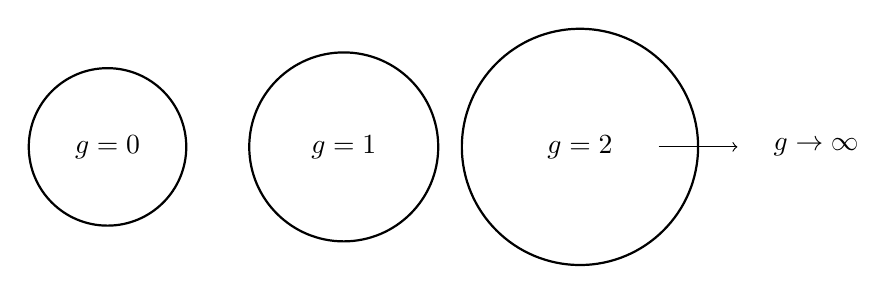
\begin{tikzpicture}
    \draw[thick] (0,0) circle (1);
    \node at (0,0) {\( g = 0 \)};
    \draw[thick] (3,0) circle (1.2);
    \node at (3,0) {\( g = 1 \)};
    \draw[thick] (6,0) circle (1.5);
    \node at (6,0) {\( g = 2 \)};
    \draw[->] (7,0) -- (8,0);
    \node at (9,0) {\( g \to \infty \)};
\end{tikzpicture}
\captionof{figure}{Perturbative Expansion of String Worldsheets}
\end{center}

\subsection{Cohomological Physics and Derived Hamiltonians}
Cohomological physics models forces, particles, and fields as projections from higher-dimensional algebraic structures. The \textbf{derived Hamiltonian} introduces higher-order corrections via cohomological resolutions:

\[
\hat{H} = \sum_i R^i H(p, q) + \int_\Sigma \mathcal{F} \wedge dA
\]
where \( R^i H \) represents cohomological corrections and \( \mathcal{F} \) describes topological forms over a surface \( \Sigma \).

\subsection{Diagram: Cohomological Projection of Derived Hamiltonian}
\begin{center}
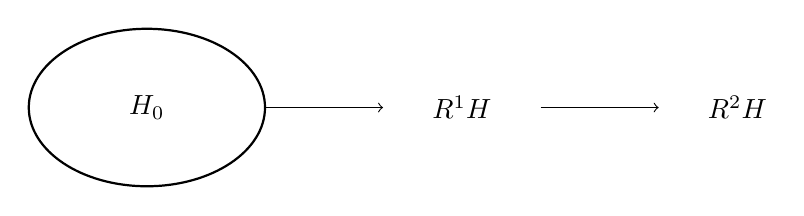
\begin{tikzpicture}
    \draw[thick] (0,0) ellipse (1.5 and 1);
    \node at (0,0) {\( H_0 \)};
    \draw[->] (1.5,0) -- (3,0);
    \node at (4,0) {\( R^1 H \)};
    \draw[->] (5,0) -- (6.5,0);
    \node at (7.5,0) {\( R^2 H \)};
\end{tikzpicture}
\captionof{figure}{Higher-Order Derived Hamiltonians via Cohomological Projection}
\end{center}

\section{Physical Implications of Derived Hamiltonians}
The derived Hamiltonian framework offers a non-perturbative alternative to string theory by modeling corrections as algebraic resolutions rather than higher-genus loops.

\subsection{Applications in Quantum Gravity}
In quantum gravity, derived Hamiltonians resolve singularities by lifting spacetime configurations into derived categories:
\[
D^b(Coh(X)) \implies \text{Resolution of Spacetime Singularities}
\]

\subsection{Applications to Topological Phases of Matter}
Spectral sequences model topological phases of matter by tracking higher-order corrections to quantum fields:
\[
E_2^{p,q} \implies E_\infty^{p+q} \implies \text{Phase Transition}
\]

\section{Strengths and Experimental Predictions}
\subsection{Advantages of Cohomological Physics}
\begin{itemize}
    \item Mathematically rigorous (derived from homological algebra).
    \item Minimal physical assumptions (avoids introducing new particles or dimensions).
    \item Non-perturbative (applies to strong-coupling regimes in quantum field theory).
\end{itemize}

\subsection{Limitations and Open Problems}
\begin{itemize}
    \item Lack of direct experimental predictions.
    \item Requires reinterpretation of physical laws through abstract mathematics.
\end{itemize}

\section{Conclusion}
Cohomological physics and derived Hamiltonians provide a rigorous alternative to string theory’s perturbative framework. While string theory offers intuitive physical narratives, the algebraic foundations of cohomological physics suggest a deeper unification across domains. Future work aims to translate these abstract mathematical structures into experimentally testable predictions.

\section{Acknowledgments}
This work was conducted under the guidance of Magneton Labs, dedicated to advancing mathematical physics and algebraic geometry.

\end{document}
